\documentclass[../main.tex]{subfiles}

\begin{document}
\section{Methods}
To determine whether GANalyze \parencite{goetschalckxGANalyzeVisualDefinitions2019} can be used to study what it means for an image to be aesthetic, I conducted a study to test whether human participants indeed preferred the images that GANalyze generated to be more aesthetic over a corresponding base image.

I used GANalyze with AestheticsNet \parencite{kongPhotoAestheticsRanking2016} as the assessor and BigGAN-256 \parencite{brockLargeScaleGAN2019} pretrained on ImageNet \parencite{russakovskyImageNetLargeScale2015} as the generator to train the GANalyze model for 400,000 iterations. The training resulted in GANalyze being able to produce image sequences based on 1,000 ImageNet categories. For each ImageNet category, I generated three different seeds (i.e., three different images of Siamese cats) to test for an effect of category. Within each seed, GANalyze produced 21 images with a supposedly increasing amount of aesthetic value (Figure ~\ref{fig:sample_sequence}). I picked a broad range of $\alpha$-values with increasing density close to zero to obtain stimuli with obvious changes (e.g., $\alpha$ = 0.25), but also subtle changes (e.g., $\alpha$ = 0.0025). I chose these values because I hypothesized the participants to agree with GANalyze 100 of the time for trials with a large $\alpha$-value, and 50 of the time (picking at random) for very small $\alpha$-values, resulting in a psychometric function. The specific $\alpha$-values were chosen based on the results of a pilot study with a very broad range.

\begin{figure}[ht]
	\caption{Truncated Sample of an Image Sequence from One Seed Produced by GANalyze}
	\label{fig:sample_sequence}
	\centering
	\begin{subfigure}{.18\textwidth}
		\centering
		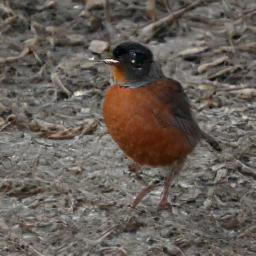
\includegraphics[width=1\linewidth]{methods/1}
		\caption{\centering $\alpha = -0.25$}
	\end{subfigure} \hfill
	\begin{subfigure}{.18\textwidth}
		\centering
		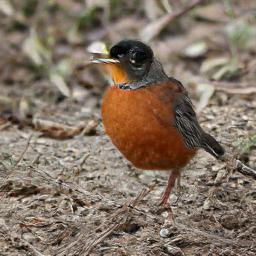
\includegraphics[width=1\linewidth]{methods/2}
		\caption{\centering $\alpha = -0.10$}
	\end{subfigure} \hfill
	\begin{subfigure}{.18\textwidth}
		\centering
		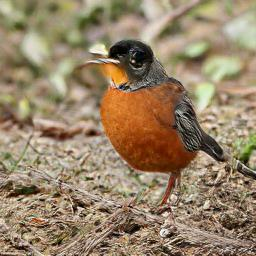
\includegraphics[width=1\linewidth]{methods/3}
		\caption{\centering $\alpha = 0$}
	\end{subfigure} \hfill
	\begin{subfigure}{.18\textwidth}
		\centering
		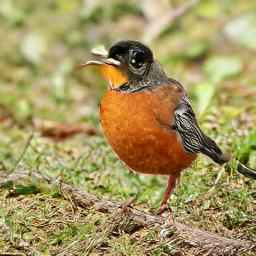
\includegraphics[width=1\linewidth]{methods/4}
		\caption{\centering $\alpha = 0.10$}
	\end{subfigure} \hfill
	\begin{subfigure}{.18\textwidth}
		\centering
		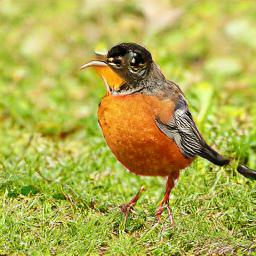
\includegraphics[width=1\linewidth]{methods/5}
		\caption{\centering $\alpha = 0.25$}
	\end{subfigure} \hfill
\end{figure}

489 ImageNet categories were manually excluded from the stimulus set because they either contained human faces (which are deliberately warped by BigGAN) or insects such as spiders which might make some participants feel uncomfortable. In addition, stimuli that were unrecognizable were also excluded. This resulted in 9xx categories, each with three seeds and 21 $\alpha$-values, equaling a total of \totalstimuli{} stimuli.

The study was hosted on Prolific.co to obtain a large number of data points in a simple online task, ensuring each of the \totalstimuli{} stimuli was evaluated 2-3 times on average. Individuals younger than 17 or those without normal or corrected-to-normal vision were not allowed to participate. At the start of the study, participants were asked to fill in demographic details such as their age, gender, and country. They were also polled on their previous experience and familiarity with visual arts. Afterwards, they had to read and accept an informed consent document after which they were provided with instructions for the task.
The participants carried out a spatial two-alternatives forced choice (2AFC) task in which they had to indicate which of the two presented GAN-generated images they considered to be most aesthetically pleasing. They did this by pressing "F" for the left, and "J" for the right image (Figure ~\ref{fig:trial_sequence}).

Each trial consisted of two images generated from the same seed within an ImageNet category. One of the two images was always the base image with $\alpha = 0$ from that trial’s seed while the comparison image was, according to GANalyze at least, either more aesthetic ($\alpha > 0$) or less aesthetic ($\alpha < 0$). The $\alpha$-value for the comparison image differed for each trial, leading to differences in similarity between the base and comparison images for each trial. An $\alpha$-value close to zero indicates high similarity and, consequently, difficulty to discriminate between the images. An $\alpha$-value much larger or smaller than zero indicates low similarity and therefore easy discrimination. The position of the base and comparison image was randomized for each trial to prevent possible confounding factors. Each 10-minute block was created to contain a roughly uniform distribution of chosen $\alpha$-values and ImageNet categories to ensure that each participant is presented with a comparable stimulus set. Furthermore, the same category never appeared more than one time in a block.

After 10 minutes, the task automatically turned to a screen thanking the participants for their assistance, after which they were given monetary compensation of £1.38 converted to their local currency.


\begin{figure}
	\centering
	\caption{Example of a Sequence of Trials in the Study}
	\label{fig:trial_sequence}
	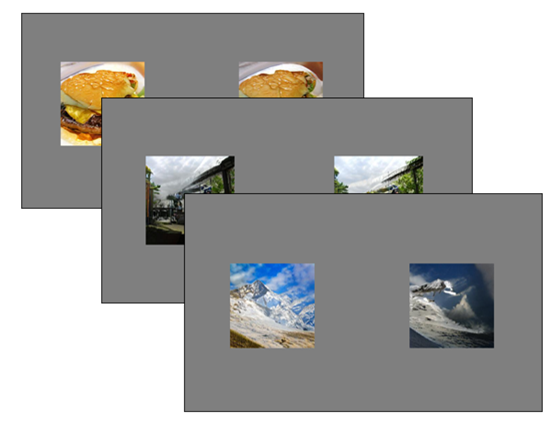
\includegraphics[scale=0.60]{trial_sequence}
\end{figure}


	\subsection{Questionnaire}
	I used a shortened version of the Aesthetic Experience Questionnaire (AEQ; \cite{wanzerExperiencingFlowViewing2020}) to measure experience and ... with art/aesthetics. I picked only the highest loading question for each of the six factors in order to save on time.

	\subsection{ss2}
	st2

	\subsection{ss3}
	Check out \textcite{goetschalckxGANalyzeVisualDefinitions2019}.

\end{document}
